\chapter{Fundamentals of Well Testing}
\label{chapter-well-testing}

This chapter will give a brief description of well testing and the diagnostic tools utilized in this project.

Well testing is commonly utilized in the industry for obtaining information about the reservoir and the well.
%
Those data are then included in reservoir models for predicting the well and field responses to different development scenarios.
%
According to \cite{Bourdet2002}, the information obtained in a well test include:
%
\begin{itemize}
\item Average horizontal and vertical permeabilities in an investigated region.
\item The presence or absence of heterogeneities in the reservoir, such as natural fractures, layering, and variation in the reservoir characteristics.
\item The presence or absence of boundaries close to the well, their distance, and shape.
\item Initial pressure in an investigated region.
\item Average pressure in an investigated region.
\item Well productivity index, or PI.
\item Well skin factor (a dimensionless pressure drop due to damage or stimulation in the interface between the well and the reservoir).
\item Well geometry.
\end{itemize}
%
Different than the static data obtained with geological and logging methods, a well test provides the reservoir proprieties in dynamic conditions.
%
Workflows of integrated reservoir characterization commonly utilize both kinds of data to build a robust model.

In a well testing operation, a change in the flow rate originates a transient in the bottom hole pressure.
%
This transient is then monitored in a usually short time period (compared to the field life cycle).
%
Commonly, the pressure is recorded down-hole with a tool, while the flow rate is controlled in the surface.
%
In the initial conditions, the bottom hole pressure, BHP, is constant.
%
After opening the well, this pressure decreases while the well produces.
%
This drawdown pressure drop, $\Delta p_{Dd}$, is described as:
%
\nomenclature[U]{Dd}{Drawdown}
\nomenclature[U]{BU}{Build up}
%
\begin{equation}
	\Delta p_{Dd} = p_i - p(t).
\end{equation}
%
When the well ceases its production, the build-up pressure change, $\Delta p_{BU}$ is:
%
\begin{equation}
	\Delta p_{BU} = p(t) - p(t=0),
\end{equation}
%
where $p(t=0)$ is the pressure in the last time recorded with the well flowing.
%
Figure \ref{figure-example-well-test} shows a typical sequence of a drawdown/build-up well test.
%
\begin{figure}[H]
	\label{figure-example-well-test}
	\centering
	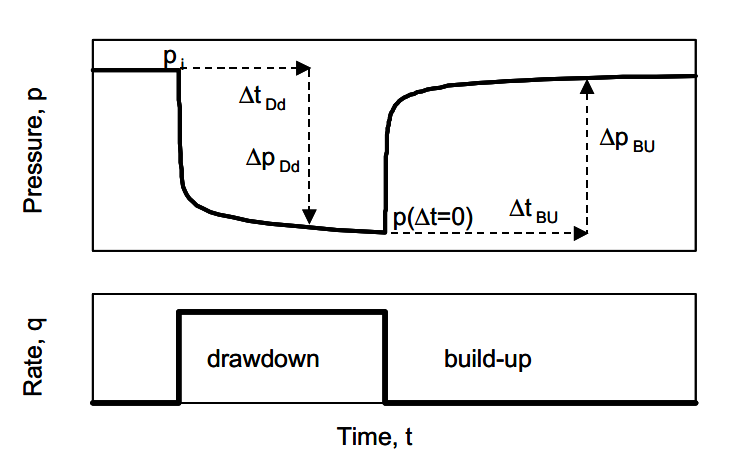
\includegraphics[width=0.8\linewidth]{figure-example-well-test.png}
	\caption{Typical representation of a bottom hole pressure behavior in a drawdown/build-up test. Source: \cite{Bourdet2002}.}
\end{figure}
\noindent
%
Besides the previous plots shown above, a log-log plot is also utilized in the post-processing of data. 
%
That helps to identify patterns that could not be seen initially. 
%
\cite{Bourdet2002} shows an example of such analysis in the diagnostic of a well in partial penetration in a reservoir.
%
Figures \ref{figure-spherical-flow} and \ref{figure-spherical-flow-diagnostic} illustrates this example.
%
\begin{figure}[H]
	\centering
	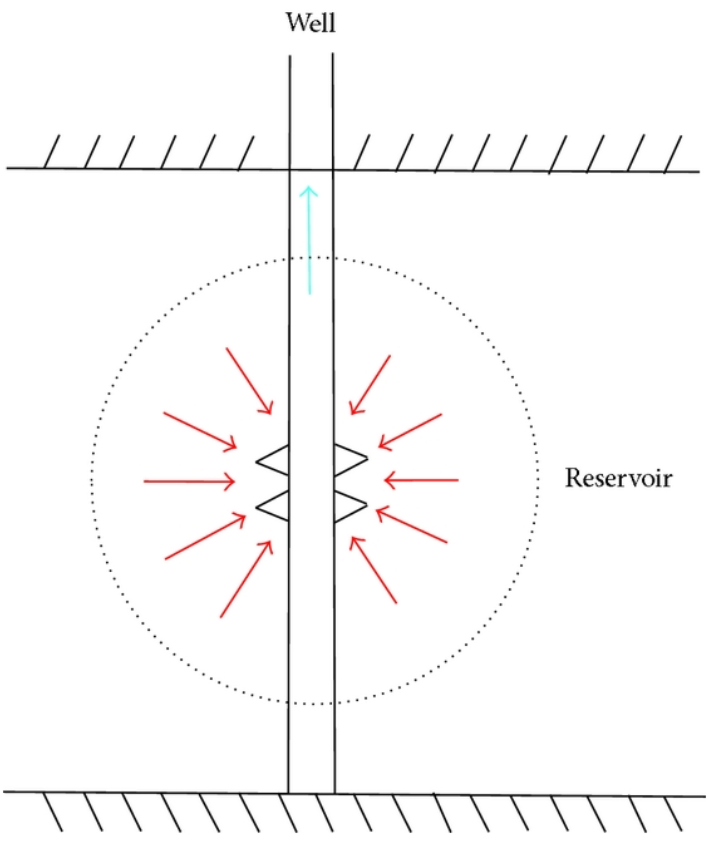
\includegraphics[width=0.5\linewidth]{figure-spherical-flow.png}
	\caption{Schematical representation of a spherical flow in a reservoir. Source: \cite{Bourdet2002}.}
	\label{figure-spherical-flow}
\end{figure}
%
\begin{figure}[H]
	\centering
	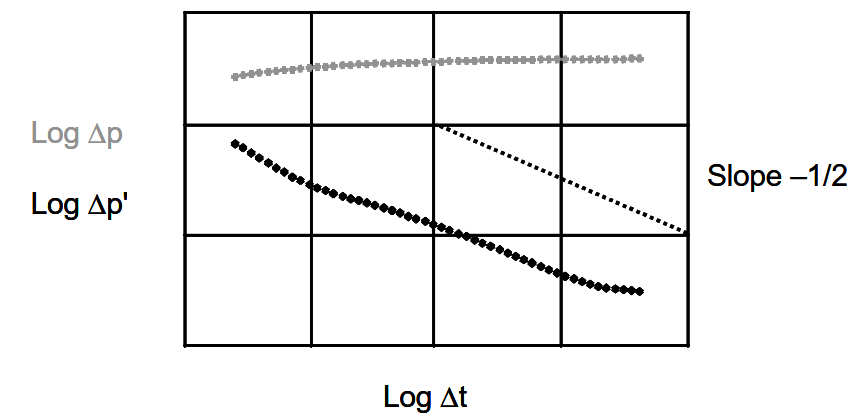
\includegraphics[width=0.9\linewidth]{figure-spherical-flow-diagnostic.png}
	\caption{Pressure drop and its derivative in a log-log plot for a well with partial penetration. \cite{Bourdet2002} shows that the slope of the pressure derivative curve is equal to $-\frac{1}{2}$ in this scenario. Source: \cite{Bourdet2002}.}
	\label{figure-spherical-flow-diagnostic}
\end{figure}
\noindent
%
This log-log diagnostic graphic plots the pressure drop and its derivative for a drawdown test.
%
The equations below show how those plots are drawn:
%
\nomenclature[R]{$p_i$}{Initial pressure in a buildup or drawdown test}
%
\begin{equation}
	\label{equation-pressure-drop}
	\Delta p_{wf} = p_{wf} - p_i,
\end{equation}
%
\begin{equation}
	\label{equation-pressure-drop_derivative}
	\frac{\partial \Delta p_{wf}}{\partial \log t} \approx \frac{\Delta p_{wf}(\log t) + \Delta p_{wf}(\Delta \log t)}{\Delta \log t},
\end{equation}
%
In the example above, the fluid enters the well by a spherical flow.
%
\cite{Bourdet2002} shows that for this situation, the Bourdet derivative curve follows a straight line with a negative half-unit slope.
%
\cite{Bourdet2002} shows several other diagnostics that could be obtained in well tests by similar analysis.
%
This project's focus is limited to evaluating how this diagnostic log-log plot will change from a model before and after its upscaling.

